%\begin{sidewaysfigure}
%  \begin{center}
%  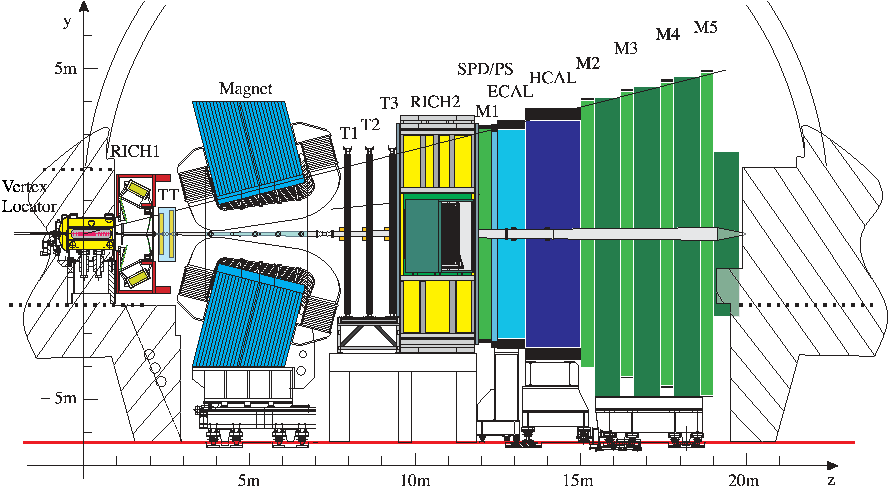
\includegraphics[width=0.8\textheight]{lhcb-detector-cross-section}
%  \caption[Cross-section view of \LHCb, cut in the non-bending $y$--$z$ plane]%
%    {Cross-section view of \LHCb, cut in the non-bending $y$--$z$ plane.}
%  \label{fig:LHCbCrossSection}
%  \end{center}
%\end{sidewaysfigure}



\chapter{Neutrino interactions with atomic nuclei}
\label{chap:NeutrinoInteractionsAtomicNuclei}
The neutrino is a strictly weakly interacting particle.  This has difficult implications for any experiment aiming to study neutrinos as particle detectors generally rely on the electromagnetic force.  In fact, the only proven method of neutrino detection is to utilise a high mass target in which the neutrinos can interact with.  Generally speaking, charged particles are produced by this interaction which can be detected by the usual means.  The collected information from these charged final states can then be used to infer information about the incident neutrino.  All neutrino experiments rely on this method and so any attempted measurements (e.g. $\delta$) rely on our understanding on neutrino interactions with atomic nuclei.  Our understanding of such processes is emcompassed in the models we use to simulate the interactions.

\section{Neutrino interactions at the GeV-scale}
\label{sec:NeutrinoInteractionsGeVScale}
As the neutrino is weakly interacting, there are two channels available to a neutrino interacting with a nucleon: the Charge Current (CC) interaction in which are W boson is exchanged and the Neutral Current (NC) interaction in which a Z boson is exchanged.  For neutrino energies below $\sim$1~GeV, the neutrino-hadron interactions are largely Quasi-Elastic (QE)~\cite{RevModPhys.84.1307}.  In such an interaction, the incident neutrino scatters of the nucleon as if it were a single particle, rather than with one of the nucleon's constituent partons.  In the case of a CCQE interaction, the neutrino is converted into its charged lepton equivalent and the target neutron converted to a proton.  In the specific case of an incident $\nu_\mu$, the interaction takes the following form
\begin{equation}
\nu_\mu n \rightarrow \mu^- p
\label{eq:CCQEInteraction}
\end{equation}
For NCQE interactions, the incident neutrino remains after the interaction has occurred and no nucleon coversion takes place.  Because of this fact, the target nucleon in a NCQE interaction need not be a neutron.  So, for $\nu_\mu$ NCQE interactions, there are two channels available
\begin{equation}
\nu_\mu n \rightarrow \nu_\mu n,
\label{eq:NCQEInteractionNeutronTarget}
\end{equation}
\begin{equation}
\nu_\mu p \rightarrow \nu_\mu p.
\label{eq:NCQEInteractionProtonTarget}
\end{equation}
The two kinds of QE interaction are shown in Fig.~\ref{fig:QEFD}.
\begin{figure}%
  \centering
  \subfloat[CCQE.]{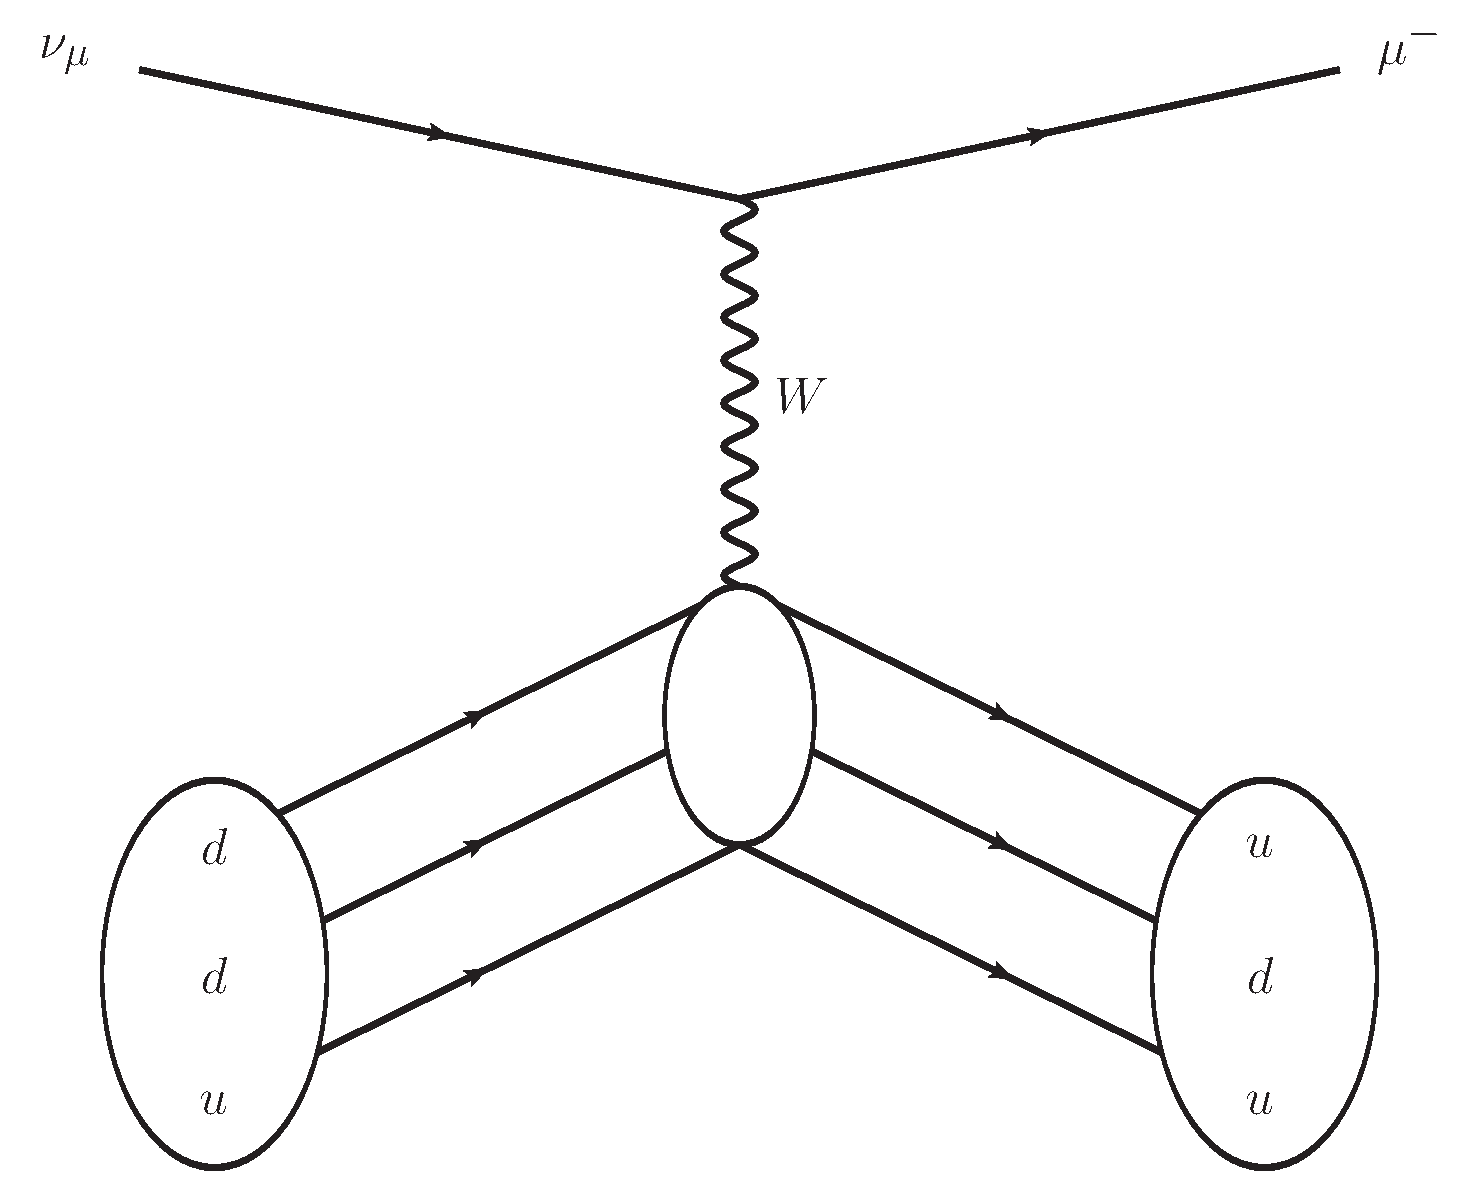
\includegraphics[width=8cm]{images/neutrino_interactions/CCQE_FD.eps} \label{fig:CCQEFD}}
  \subfloat[NCQE.]{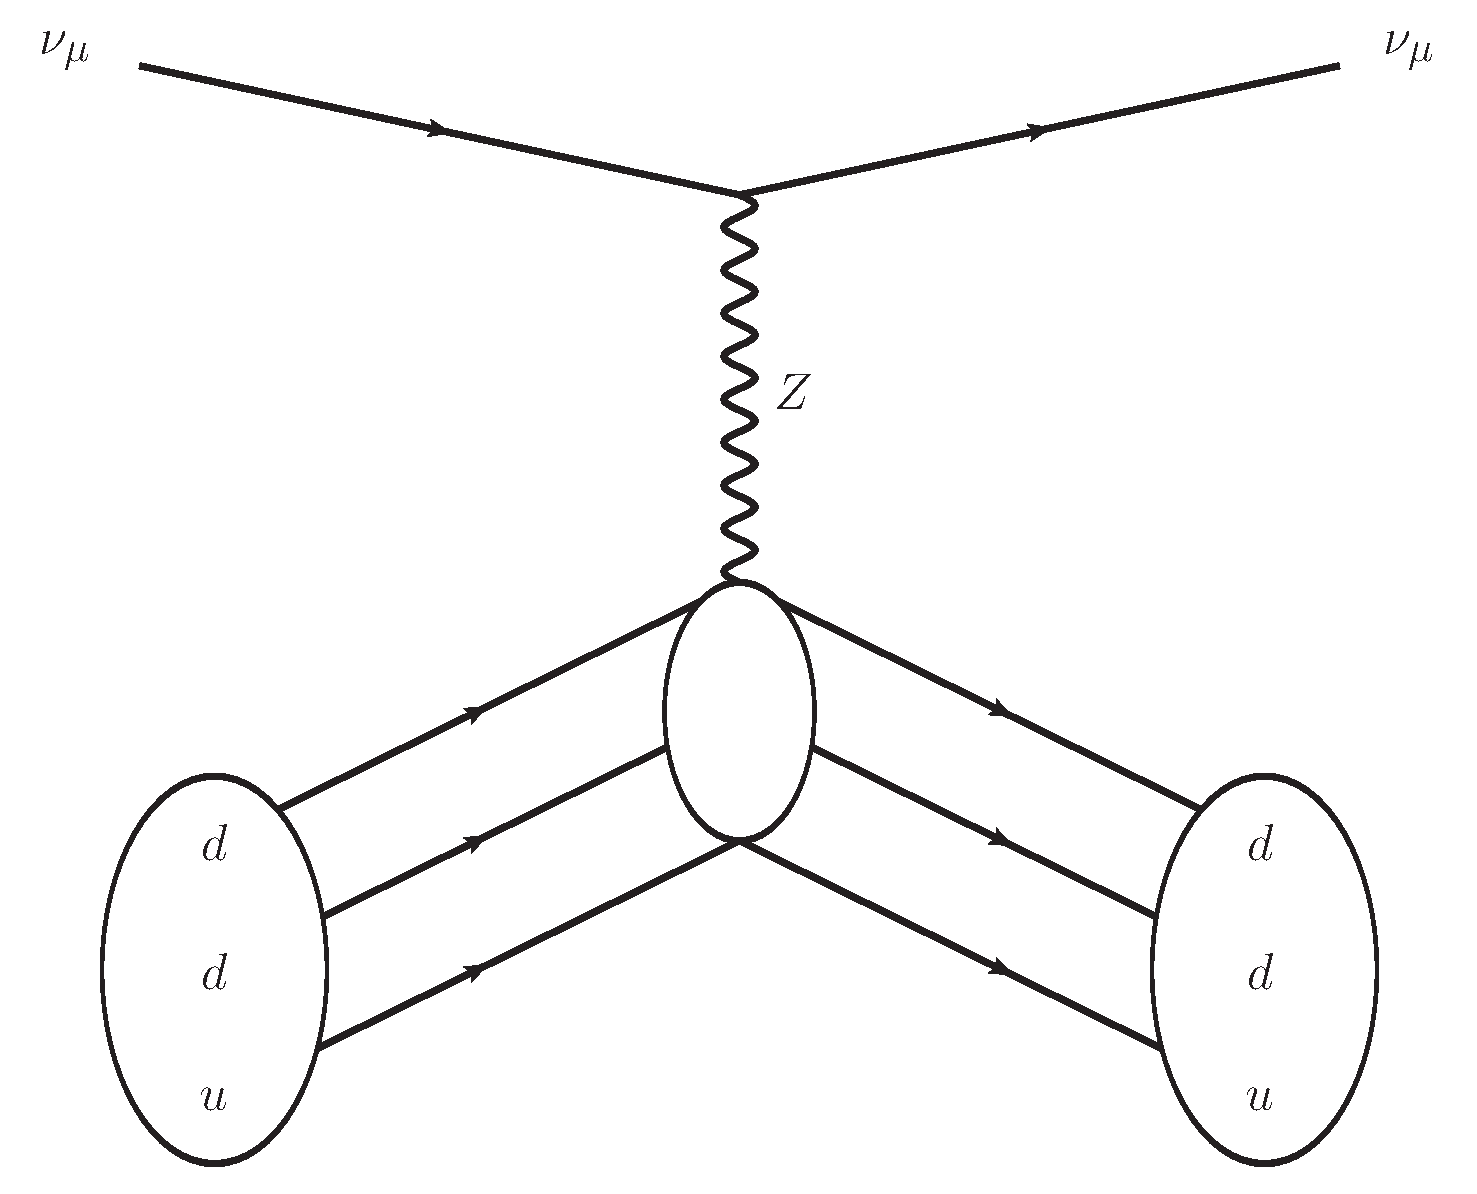
\includegraphics[width=8cm]{images/neutrino_interactions/NCQE_FD.eps} \label{fig:NCQEFD}}
  \caption{Quasi-Elastic (QE) interactions of a $\nu_\mu$ with a nucleon.  The small ellipse represents the neutrino interacting with the nucleon as a whole, rather than with an individial parton.}
  \label{fig:QEFD}
\end{figure}
\newline
\newline
For higher energy neutrinos, there is sufficient energy to promote the target nucleon to an excited state.  A quick after-effect of this promotion is that the excited state decays, resulting in further particle emission.  This interaction topology, which dominates in the 1~GeV to 5~GeV energy range, is known as RESonant pion (RES) production as the neutrino interaction produces $\Delta$ resonance which typically decays to a nucleon and a single pion in the final state.  In the case of $\nu_\mu$ CCRES, the interaction generally takes the following form
\begin{equation}
\nu_\mu N \rightarrow \mu^- N^{*},
\label{eq:CCRES}
\end{equation}
\begin{equation}
N^{*} \rightarrow \pi N',
\end{equation}
where $N, N' = n, p$.  An example diagram of $\nu_\mu$-CCRES interaction with a $\pi^+$ in the final state is shown in Fig.~\ref{fig:CCRESFD}.
\begin{figure}%
  \centering
  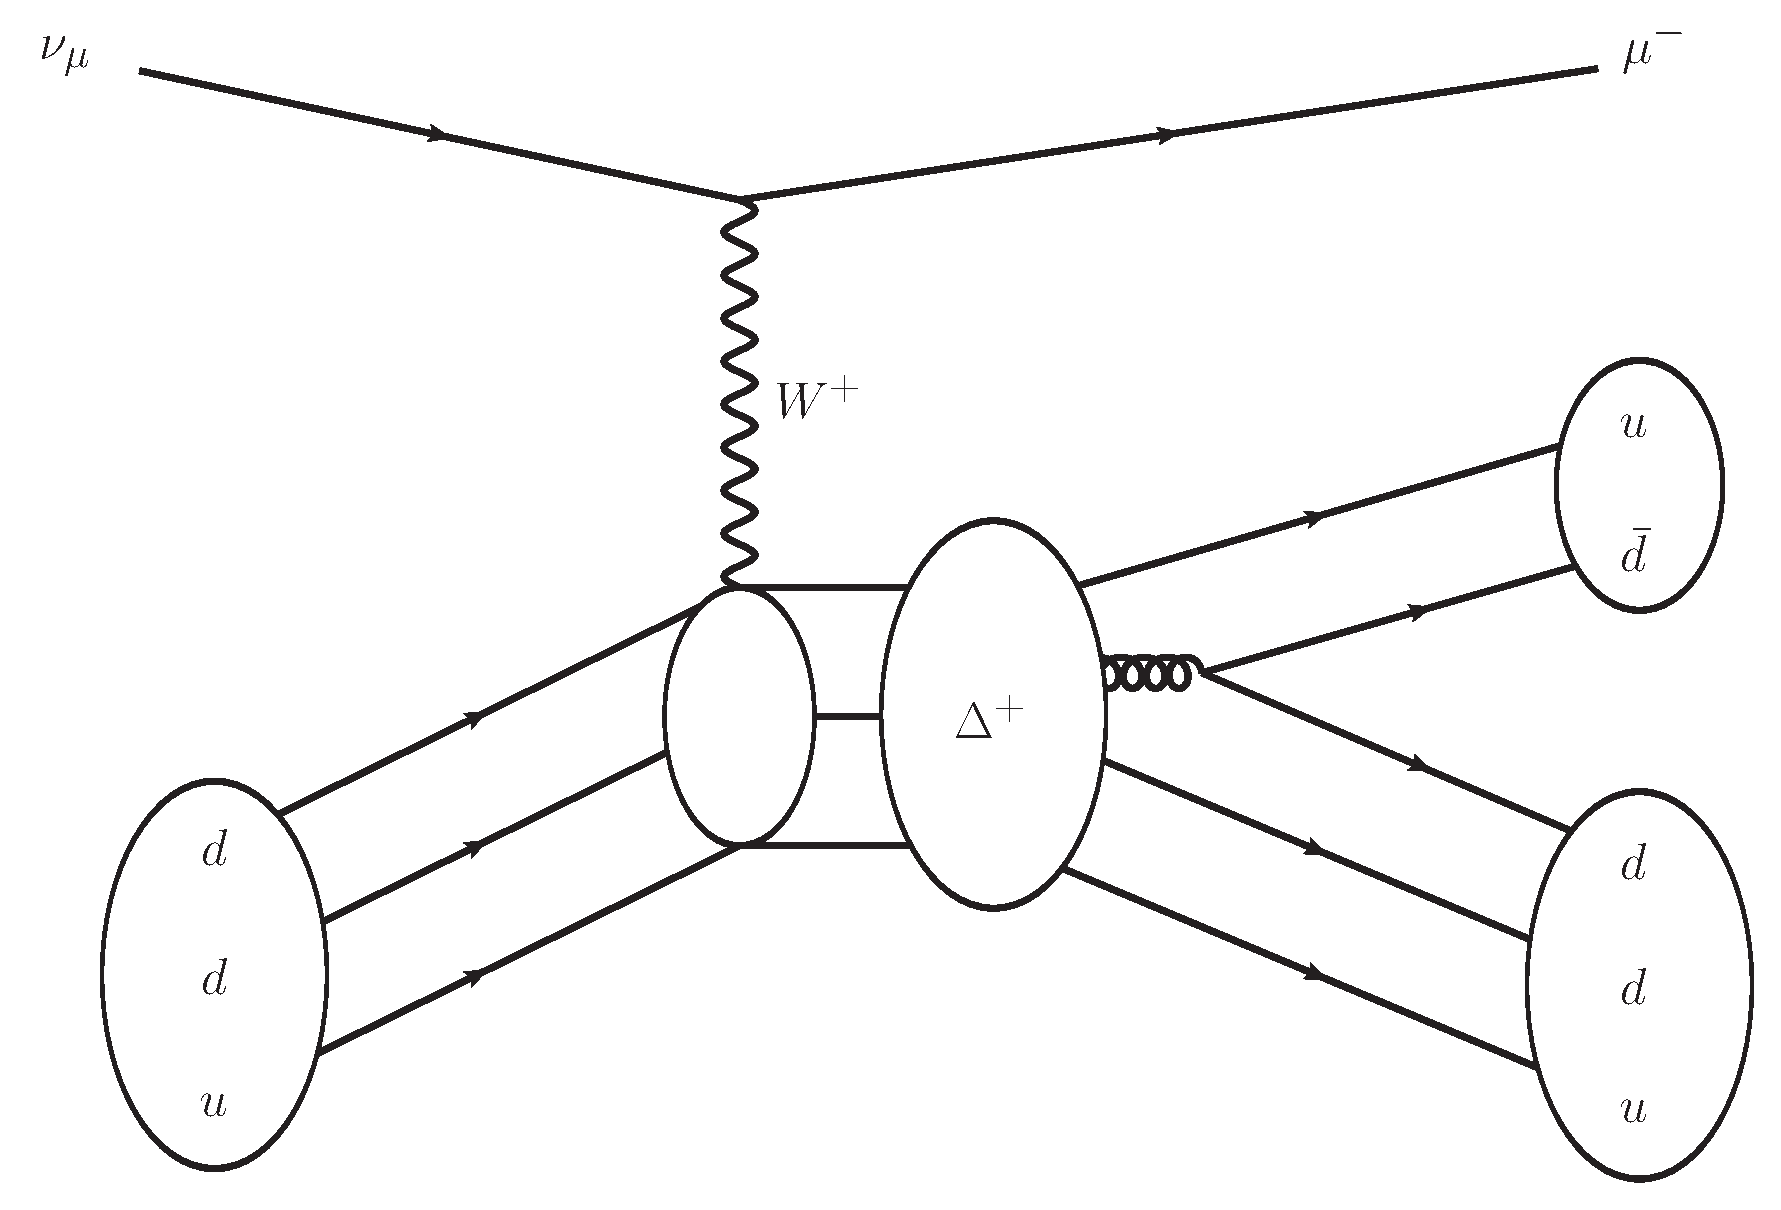
\includegraphics[width=8cm]{images/neutrino_interactions/CCRES_FD.eps}
  \caption{A Charged Current RESonant pion (CCRES) interaction of a $\nu_\mu$ with a neutron.  The $\Delta$ resonance decays to a neutron and a $\pi^+$.}
  \label{fig:CCRESFD}
\end{figure}
\newline
\newline
For neutrinos with energy above the RES-dominant region, the neutrino has enough energy to penetrate the nucleon and scatter off an individual quark.  Because of the nature of the strong force, the scattered quark, and the nucleon remnant, produce a hadronic shower in the final state.  This process is known as Deep Inelastic Scattering (DIS).  For $\nu_\mu$-CCDIS, the interaction takes the following form
\begin{equation}
\nu_\mu N \rightarrow \mu^- X,
\label{eq:CCDIS}
\end{equation}
where $X$ is the remnant of the nucleus after the interaction occurs.  An example diagram of a $\nu_\mu$-CCDIS interaction is shown in Fig.~\ref{fig:CCDISFG}.
\begin{figure}%
  \centering
  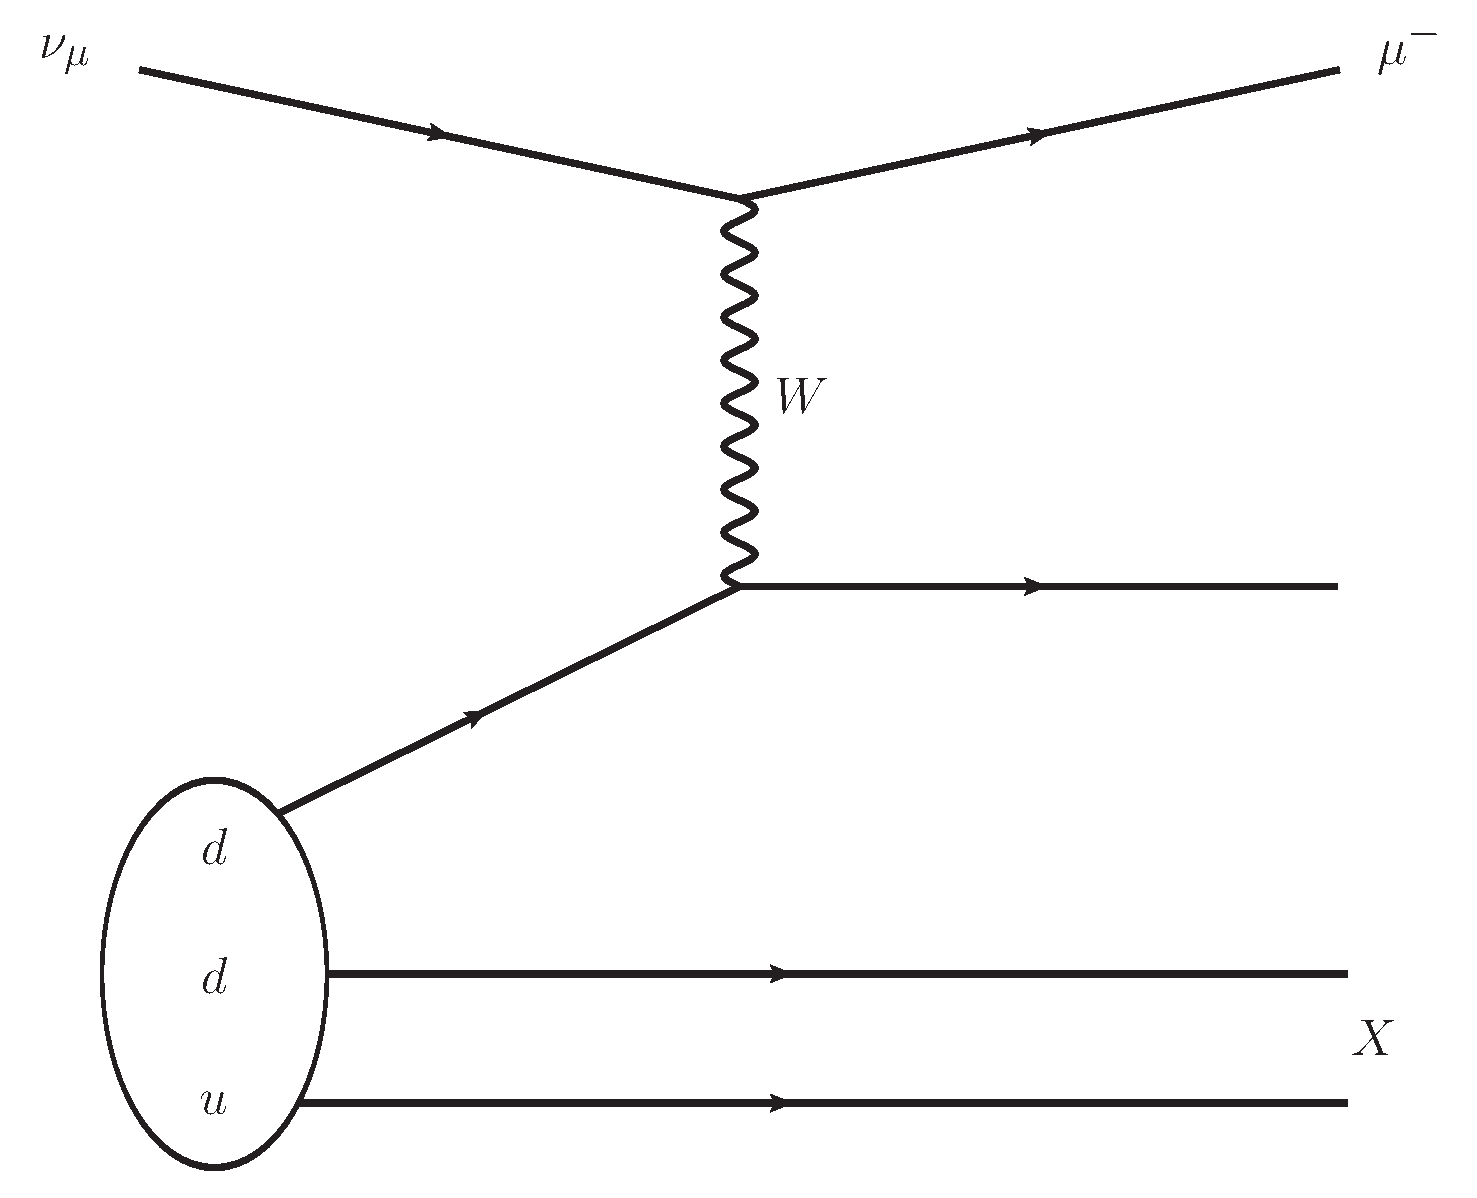
\includegraphics[width=8cm]{images/neutrino_interactions/CCDIS_FD.eps}
  \caption{A Charged Current Deep Inelastic Scattering (CCDIS) interaction of a $\nu_\mu$ with a neutron. $X$ resembles the leftover nuclear remnant.}
  \label{fig:CCDISFG}
\end{figure}
\newline
\newline
While the value of a particular interaction cross-section should depend on the nuclear environment, it is possible to make comparisons of the measured cross-section per nucleon.  Fig.~\ref{fig:CrossSectionMeasurements} shows a comparison of $\nu_\mu$ CC cross-section measurements per nucleon from different experiments, all of which sample a different neutrino energy range.  There are large uncertainties for many of the cross-section meausrements, particularly for the ones sampling the lower energy ranges.  The T2K beam energy is $\sim$700~MeV, which sits in the region of higher uncertainty.
\begin{figure}%
  \centering
  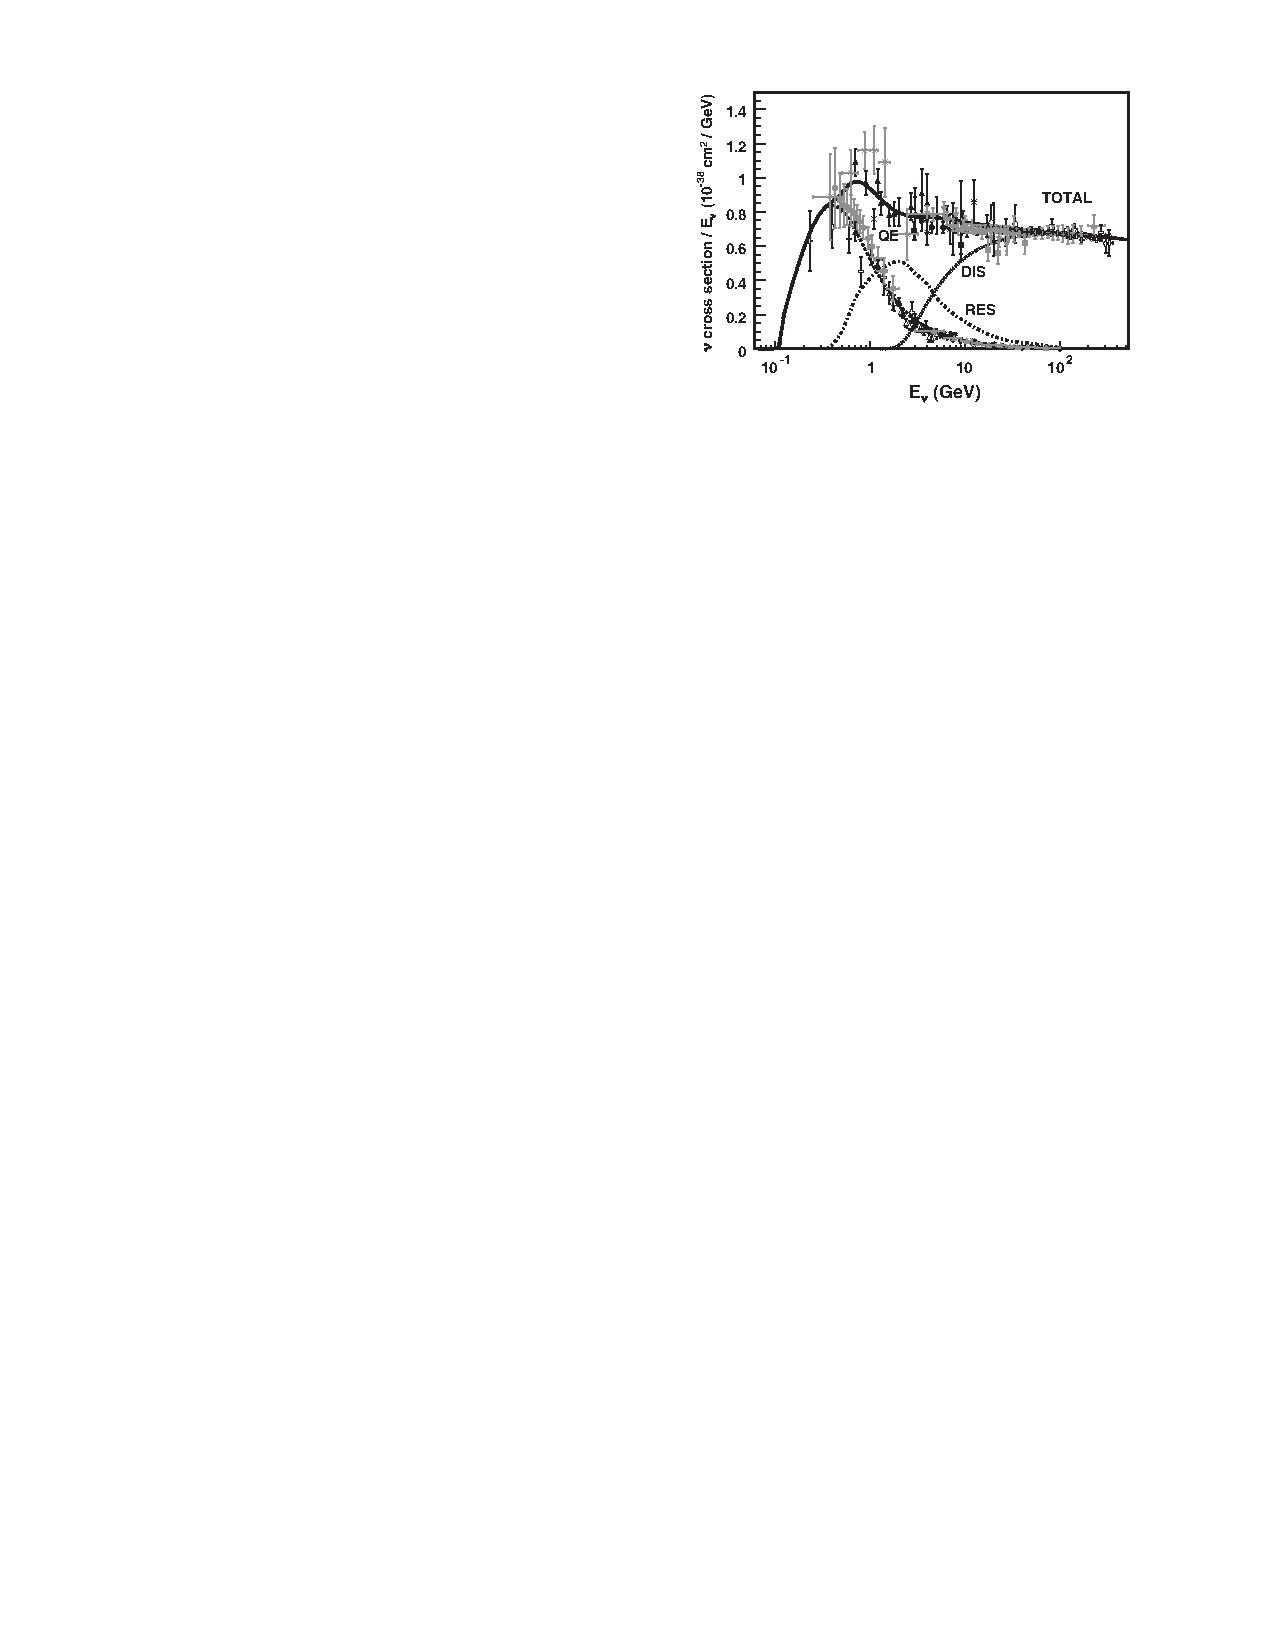
\includegraphics[width=8cm]{images/neutrino_interactions/CrossSectionMeasurements.pdf}
  \caption{$\nu_mu$ CC cross-section measurements per nucleon for a range of energies, showing the QE, RES and DIS contributions~\cite{RevModPhys.84.1307}.}
  \label{fig:CrossSectionMeasurements}
\end{figure}
\newline
\newline
CCQE interactions are, experimentally, the most interesting and this is the interaction region where most recent measurements have been focused.  Because of the simplicity of the CCQE topology, the interaction can be treated as a two-body scatter.  So, by applying simple conservation rules, the neutrino energy can be kinematically reconstructed.  In such interactions, the nucleon structure is parameterised using a set of form factors, the most interesting of which is the axial-vector form factor, $F_A(Q^2)$. $F_A(Q^2)$ has been, and still is, assumed to take a dipole form
\begin{equation}
F_A(Q^2) = \frac{F_A(0)}{(1-Q^2/M_A^2)^2}
\label{eq:FAFormFactor},
\end{equation}
where $Q^2$ is the negative of the squared four-momentum transfer of the lepton to the hadron, $F_A(0) = 1.2694\pm0.0028$~\cite{0954-3899-37-7A-075021}, and $M_A$ is known as the axial mass.  Recent measurements of the CCQE cross-section by the MiniBooNE~\cite{PhysRevD.81.092005} and NOMAD~\cite{NOMAD-CCQE} experiments have sparked interest by reporting measured cross-sections which are in tension with one another, the results of which shown in Fig.~\ref{fig:CCQECrossSectionMiniBooNENOMAD}.  
\begin{figure}%
  \centering
  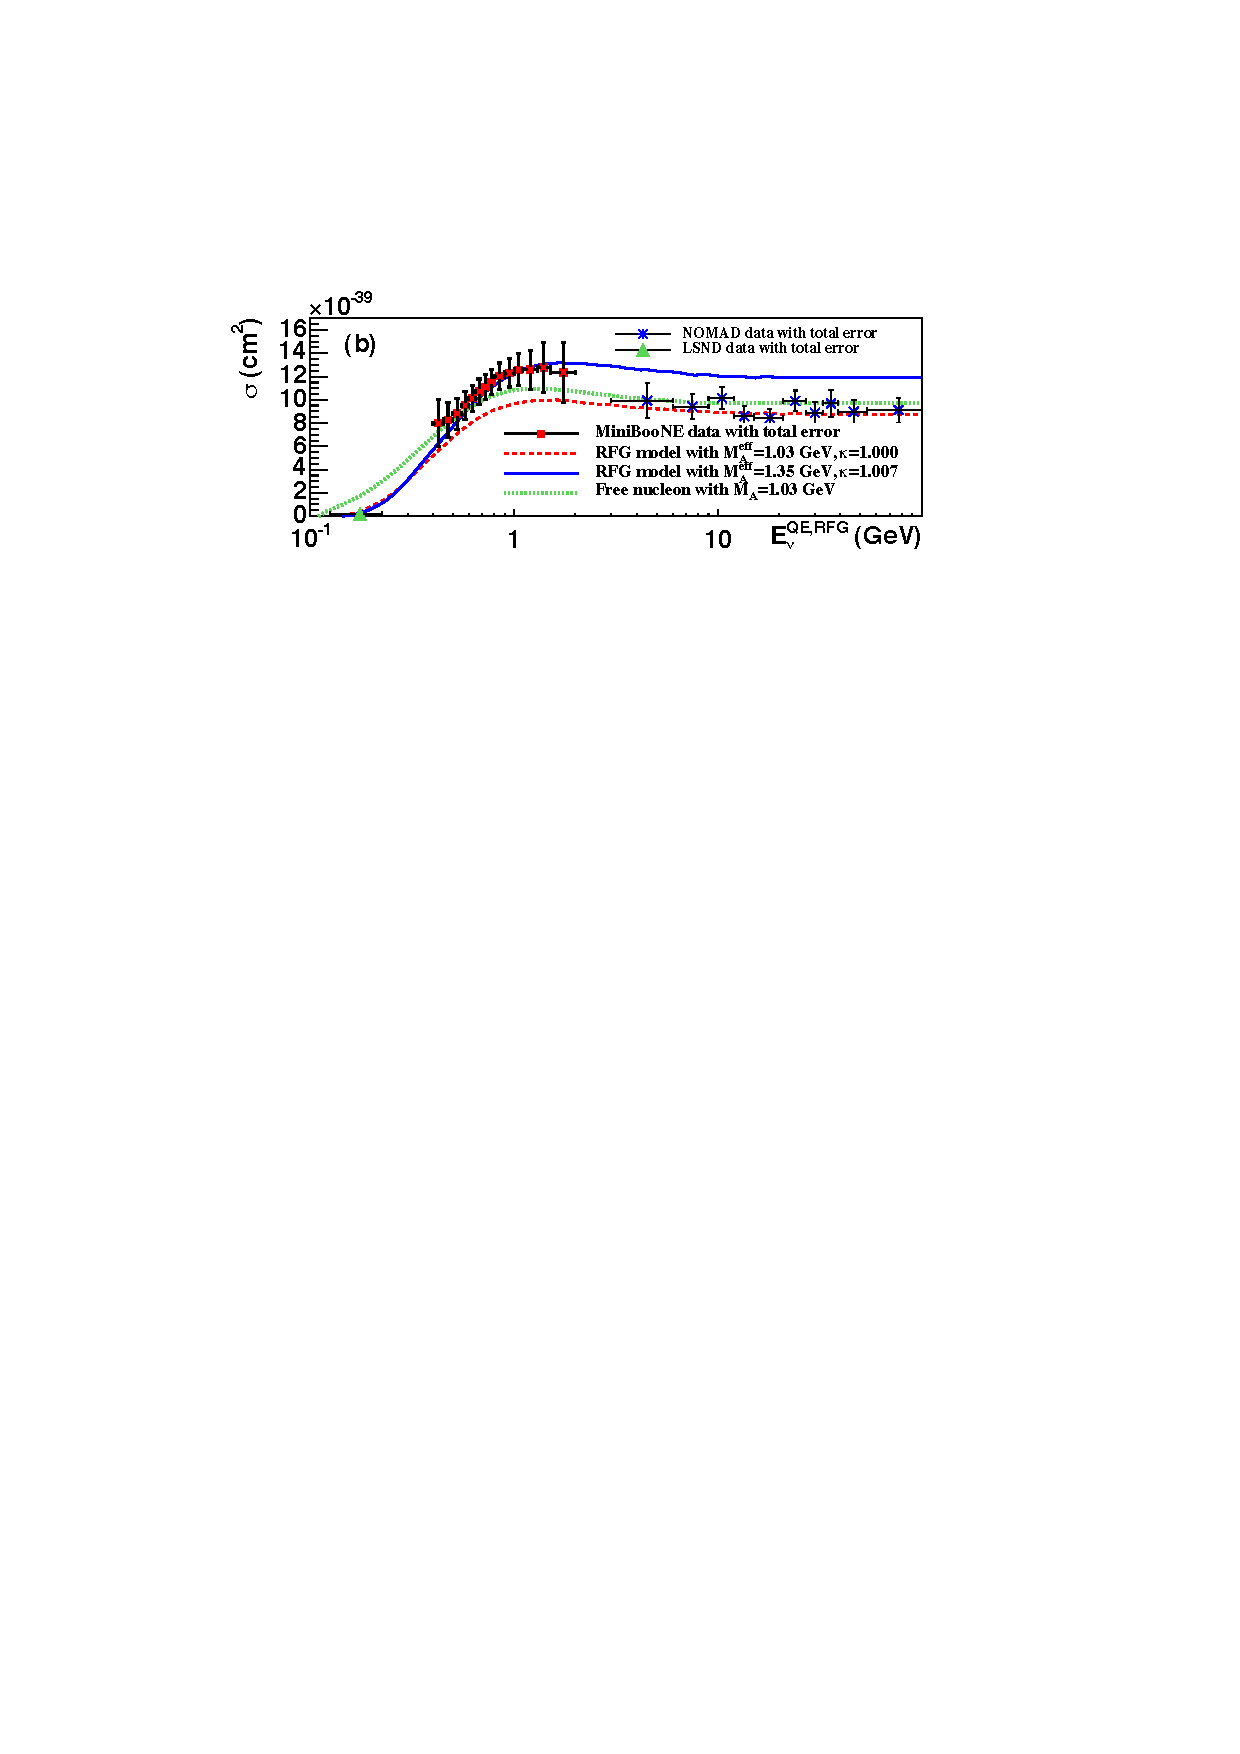
\includegraphics[width=12cm]{images/neutrino_interactions/CCQECrossSectionMiniBooNENOMAD.pdf}
  \caption{The CCQE cross-sections measured by the MiniBooNE and NOMAD experiments.  The solid and dashed lines represent models with different values of $M_A$~\cite{PhysRevD.81.092005}.}
  \label{fig:CCQECrossSectionMiniBooNENOMAD}
\end{figure}
A popular explanation for this discrepancy is a lack of understanding of the nuclear environment.  Because the neutrino is not scattering of a free nucleon, but rather a nucleon in a strongly contained system, experiments actually measure an effective $M_A$.  It is possible that the nuclear effects cause a modification to the effective $M_A$ that the experiments measure.  This possible explanation has placed a heavier emphasis on nuclear modelling in neutrino interaction experiments. 





